SHA-3 ("\textit{Secure Hash Function}"-3) ist eine vom US-amerikanischen "National Institute of Standards and Technology"
definierte Familie von kryptographischen Hashfunktionen. Zu ihr gehören SHA3-224, SHA3-256, SHA3-384, SHA3-512,
sowie noch zwei Zufallsfunktionen mit variabler Ausgabelänge SHAKE128 und SHAKE256, die wir hier aber nicht weiter betrachten wollen.
In Tabelle \ref{tab:uebersicht_sha3} sind ein paar wichtige Eigenschaften der unterschiedlichen SHA3-Funktionen aufgelistet.\\

\begin{table}
	\centering
	\begin{tabular}{lrrr}
		Name & Kapazität $c$ & Blocklänge $r$ & Hash-Länge \\
		\hline
		SHA3-224 & 448 Bit & 1152 Bit & 224 Bit \\
		SHA3-256 & 512 Bit & 1088 Bit & 256 Bit \\
		SHA3-384 & 768 Bit & 832 Bit & 384 Bit \\
		SHA3-512 & 1024 Bit & 576 Bit & 512 Bit
	\end{tabular}
	\caption{Übersicht über die verschiedenen SHA-3 Hashfunktionen}
	\label{tab:uebersicht_sha3}
\end{table}

Bei einer kryptographischen Hashfunktion handelt es sich um eine Funktion, die zu einer Eingabe beliebiger Länge
eine Art Prüfsumme mit fixer Länge berechnet, den sogenannten Hash. 
Es soll einfach sein so einen Hash für eine Eingabe zu berechnen, aber zu einem Hash eine Eingabe zu finden,
die diesen Hash besitzt, oder eine Nachricht zu verändern, sodass der Hash sich nicht verändert, soll praktisch nicht möglich sein.
Damit eine solche Hashfunktion $H$ als kryptographisch sicher gilt, erwartet man folgende grundlegende Eigenschaften von ihr:
\begin{enumerate}
    \item Einwegfunktion:\\
    Für einen gegebenen Hash h kann nicht effizient eine Nachricht M gefunden werden, sodass $H(M) = h$.
	\item Schwache Kollisionsresistenz: \\
    Zu einer gegebenen Nachricht $M$ soll es nicht möglich sein, effizient eine zweite Nachricht $M^\prime$ zu finden,
    die den gleichen Hash besitzt, sodass $H(M) = H(M^\prime)$ gilt.
	\item Starke Kollisionsresistenz: \\
    Es soll nicht möglich sein, effizient zwei Nachrichten $M$ und $M^\prime$ zu finden, die denselben Hashwert besitzen,
    also $H(M) = H(M^\prime)$ \cite{rogaway2004crypto}
\end{enumerate}
Ob eine Hashfunktion nun diese Anforderungen erfüllt, hängt davon ab, welche Mächtigkeit man einem Angreifer erlaubt,
der versucht diese Probleme zu lösen. Für klassische Computer betrachtet man typischerweise Algorithmen aus der Komplexitätsklasse $BPP$ (Bounded-Error Probabilistic Polynomial Time).
Diese Algorithmen sind probabilistisch und müssen nur mit einer Wahrscheinlichkeit von $p > 2/3$ das richtige Ergebnis ausgeben.
Es ist die mächtigste Klasse klassisch probabilistischer Algorithmen, weshalb man die Angreifer aus dieser Klasse wählt.
Quantencomputer sind jedoch in einigen Aspekten deutlich mächtiger als klassische Computer und auch wenn sie bisher
noch um mehrere Größenordnungen zu klein sind, um moderne Hashfunktionen zu brechen, untersucht man schon länger die Sicherheit
von kryptographischen Systemen wie Hashfunktionen oder Verschlüsselungen gegen Quantenalgorithmen. Analog zur Komplexitätsklasse $BPP$
gibt es daher für Quantenalgorithmen die Klasse $BQP$ (Bounded Error Quantum Polynomial Time). In \ref{cha:sha3_sicherheit} werden wir uns die
Sicherheitseigenschaften von SHA-3 genauer anschauen. \\

Um Anfragen beliebiger Länge bearbeiten zu können, bestehen Hashfunktionen typischerweise aus vier Teilen. Mit Hilfe einer \textit{Padding}-Funktion wird die Eingabe so erweitert,
dass die Länge ein ganzzahliges Vielfaches einer von der Hashfunktion benötigten Blocklänge ergibt. Die Eingabe kann so in mehrere gleich große Blöcke eingeteilt werden,
die nacheinander weiterverarbeitet werden. Aus einer \textit{Kompressionsfunktion} oder, wie im Fall von SHA-3, einer \textit{Permutation} wird dann eine Funktion konstruiert,
die nacheinander die Blöcke mit dem Ergebnis der Kompression/Permutation kombiniert und weiterverarbeitet. Während viele bekannte Hashfunktionen dazu auf
die Merkle-Damg\r{a}rd-Konstruktion zurückgreifen, verwendet SHA-3 die sogenannte \textit{Schwammkonstruktion}.
Wie diese genau aussieht und wie sie funktioniert, werden wir später in Abschnitt \ref{cha:schwammkonstruktion} sehen.

\newcommand{\bigcomp}{%
  \DOTSB
  \mathop{\vphantom{\sum}\mathpalette\bigcomp@\relax}%
  \slimits@
}
\newcommand{\bigcomp@}[2]{%
  \begingroup\m@th
  \sbox\z@{$#1\sum$}%
  \setlength{\unitlength}{0.9\dimexpr\ht\z@+\dp\z@}%
  \vcenter{\hbox{%
    \begin{picture}(1,1)
    \bigcomp@linethickness{#1}
    \put(0.5,0.5){\circle{1}}
    \end{picture}%
  }}%
  \endgroup
}
\newcommand{\bigcomp@linethickness}[1]{%
  \linethickness{%
      \ifx#1\displaystyle 2\fontdimen8\textfont\else
      \ifx#1\textstyle 1.65\fontdimen8\textfont\else
      \ifx#1\scriptstyle 1.65\fontdimen8\scriptfont\else
      1.65\fontdimen8\scriptscriptfont\fi\fi\fi 3
  }%
}

\section{Keccak-Permutation}
Als Grundlage für alle SHA3-Funktionen dient eine Instanz der Keccak-Permutationsfamilie KECCAK-p.
Für eine kryptographische Sicherheitsanalyse betrachtet man in der Regel das asymptotische Laufzeitverhalten eines Angreifers.
Hierzu benötigt man eine Funktion mit variablem Sicherheitsparameter, damit diese Analyse durchgeführt werden kann.
Wir interessieren uns hier allerdings nur für die konkrete Instanz mit einem festen Sicherheitsparameter, die vom SHA-3-Standard \cite{sha3-standard}
für die in Tabelle \ref{tab:uebersicht_sha3} aufgeführten Hashfunktionen festgelegt wird.
Die genaue Definition mit variablem Sicherheitsparameter ist zum Nachlesen auch im Standard \cite{sha3-standard} aufgeführt.
Wir wollen uns nun zuerst einmal den Zustandsvektor ein wenig genauer anschauen, auf dem die Permutation arbeitet,
bevor wir uns die fünf Unterfunktionen ansehen, aus denen die KECCAK-p-Funktion aufgebaut ist.

\subsection{Zustandsvektor}
Die KECCAK-p-Funktion arbeitet auf einem 1600 Bit breiten Zustandsvektor, der \textit{State Array} genannt wird.
Am besten lässt sich ein solches State Array \textbf{A} als einen dreidimensionalen Block aus 5x5x64 Bits vorstellen, siehe Abbildung \ref{fig:statearray}.
Wir können dabei jedes Bit von \textbf{A} über die drei Indizes $x$, $y$ und $z$ identifizieren.
Genauer gilt
\begin{align*}
    \textbf{A}[x][y][z] \in \{0,1\} (\forall x, y \in \{0,...,4\};\ z \in \{0,...,63\})
\end{align*}
Außerdem nennen wir
\begin{align*}
    & \textbf{A}[x][y] && \coloneq (\textbf{A}[x][y][0], ... , \textbf{A}[x][y][63]) && \text{ eine \textit{Lane} von \textbf{A},} \\
    & \textbf{A}[.][x][y] && \coloneq (\textbf{A}[0][y][z], ... , \textbf{A}[4][y][z]) && \text{ eine \textit{Zeile} von \textbf{A},} \\
    & \textbf{A}[x][.][z] && \coloneq (\textbf{A}[x][0][z], ... , \textbf{A}[x][4][z]) && \text{ eine \textit{Spalte} von \textbf{A},} \\
    & \textbf{A}[.][.][z] && \coloneq (\textbf{A}[.][0][z], ... , \textbf{A}[.][4][z]) && \text{ einen \textit{Slice} von \textbf{A}}
\end{align*}
\begin{figure}
	\center
	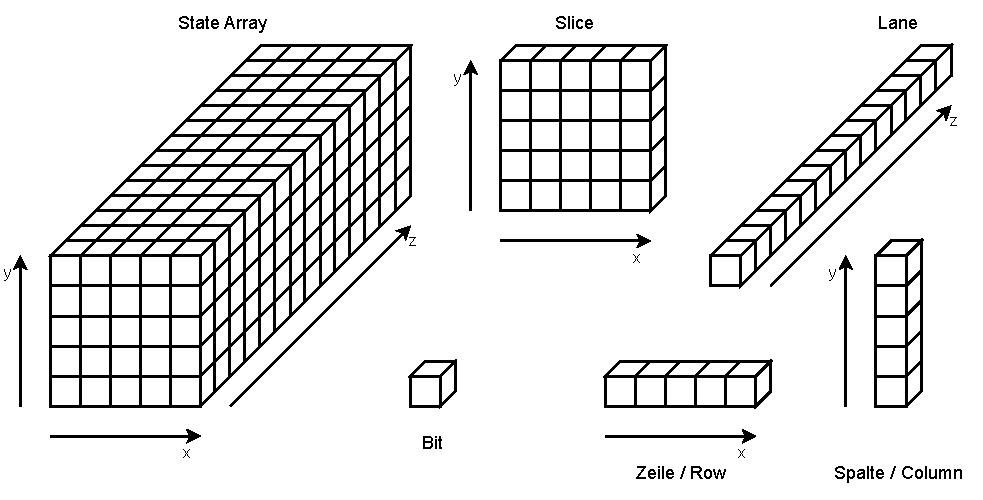
\includegraphics{images/StateArrayBeschreibung.pdf}
	\caption{Blockrepräsentation des State Array}
	\label{fig:statearray}
\end{figure}
Über die folgende Konvention können ein eindimensionaler Bitvektor $\textbf{V} \in \{0,1\}^{1600}$ und ein State Array \textbf{A} ineinander umgewandelt werden:
\begin{align*}
	\textbf{A}[x][y][z] \coloneq \textbf{V}[64(5y + x) + z] & \forall x,y = 0,...,4; z = 0,...,63
\end{align*}
Die Lanes werden also der Reihe nach erst in x-Richtung und dann in y-Richtung mit dem Inhalt von \textbf{V} gefüllt.

\subsection{Unterfunktionen}
\label{cha:sha3_unterfunktionen}
Die KECCAK-p-Funktion ist aus einer Rundenfunktion $Rnd$ aufgebaut, die mehrfach hintereinander ausgeführt wird.
Diese Rundenfunktion ist wiederum aus fünf Unterfunktionen aufgebaut, die alle auf dem State Array arbeiten.
Alle folgenden Funktionen basieren auf den Definitionen im SHA-3-Standard \cite{sha3-standard}.

\subsubsection{Theta-Unterfunktion}
\begin{figure}
    \center
    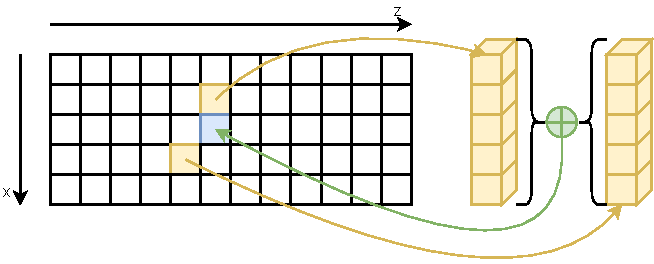
\includegraphics{images/theta.pdf}
    \caption{Spaltensummierung der $\theta$-Funktion}
    \label{fig:definition_theta}
\end{figure}
Die erste Unterfunktion der Rundenfunktion ist Theta ($\theta$). Sie modifiziert jedes Bit eines State Arrays,
indem sie, wie in Abbildung \ref{fig:definition_theta} skizziert, zwei benachbarte Spalten auf das Bit aufsummiert.
Das Symbol $\oplus$ steht dabei für die XODER-Verknüpfung und $rotl(x, k)$ beschreibt eine Linksrotation
einer Lane $x$ um eine Distanz $k$, wobei das MSB mit $z = 63$ und das LSB mit $z = 0$ indiziert wird.
\begin{align*}
    \theta (\textbf{A}) & \coloneq \textbf{A}^\prime \text{ mit } \\
    \textbf{C}[x] & \coloneq \textbf{A}[x][0] \oplus ... \oplus \textbf{A}[x][4] && \forall x = 0,...,4 \\
    \textbf{D}[x] & \coloneq \textbf{C}[(x - 1) mod\ 5] \oplus rotl(C[(x + 1) mod\ 5], 1)\ && \forall x = 0,...,4 \\
    \textbf{A}^\prime[x][y] & \coloneq \textbf{A}[x][y] \oplus \textbf{D}[x]\ && \forall x = 0,...,4;\ y = 0,...,4
\end{align*}
Die Hilfsvariable \textbf{C} hält hierbei für alle $x$ jeweils eine Lane, die an jeder Stelle die Summe aller Bits
der entsprechenden Spalte enthält. In \textbf{D} werden für alle x immer zwei Lanes an Spaltensummen aufaddiert, wobei immer
eine Lane um eine Stelle verschoben wird um das in \ref{fig:definition_theta} beschriebene Muster zu erhalten.

\subsubsection{Rho-Unterfunktion}
\begin{figure}
    \center
    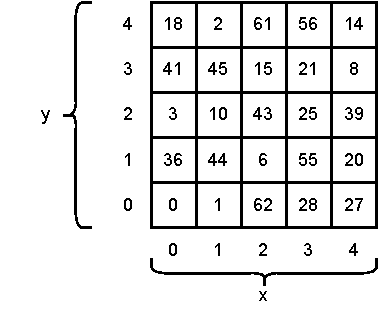
\includegraphics{images/rho.pdf}
    \caption{Rotationsdistanzen der Lanes für $\rho$}
    \label{fig:definition_rho}
\end{figure}
Bei der Rho-Unterfunktion ($\rho$) handelt es sich um eine einfache Bitrotation der einzelnen Lanes.
Bis auf die Lane bei $x=0 \text{ und } y=0$ werden alle Lanes um eine konstante Distanz nach links rotiert.
Die genauen Distanzen sind in Abbildung \ref{fig:definition_rho} aufgeführt.
\begin{align*}
    \rho (\textbf{A}) & \coloneq \textbf{A}^\prime \text{ mit } \\
    \textbf{A}^\prime[x][y] & \coloneq rotl(\textbf{A}[x][y], \textbf{D}[x][y])\ \forall x = 0,...,4;\ y = 0,...,4 \\
    \textbf{D} & :\text{ Eine 5x5 Matrix an Konstanten, siehe Abb. \ref{fig:definition_rho}}
\end{align*}

\subsubsection{Pi-Unterfunktion}
\begin{figure}
    \center
    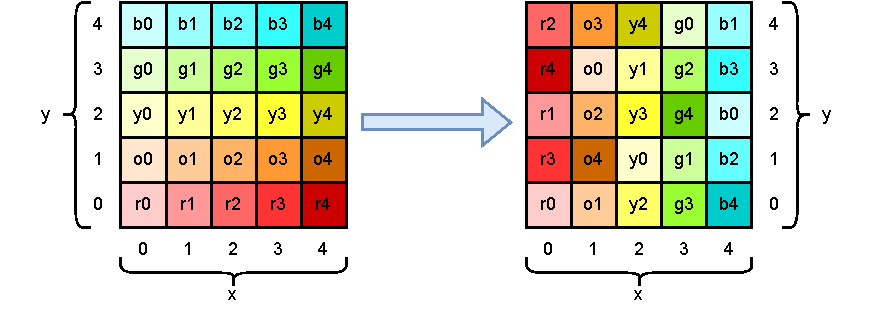
\includegraphics{images/pi.pdf}
    \caption{Visualisierung der $pi$-Permutation}
    \label{fig:definition_pi}
\end{figure}
Die Pi-Unterfunktion ($\pi$) vertauscht die Lanes eines State Arrays untereinander nach einer einfachen Vorschrift:
\begin{align*}
    \pi (\textbf{A}) & \coloneq \textbf{A}^\prime \text{ mit } \\
    \textbf{A}^\prime[x][y] & \coloneq \textbf{A}[(x + 3y)\ mod\ 5][x]\ \forall x = 0,...,4;\ y = 0,...,4
\end{align*}
Da der Ring $\mathbb{Z}/5\mathbb{Z}$ nullteilerfrei ist, ist die Indexberechnung $(x + 3y)\ mod\ 5$ injektiv für ein festes $x$.
Es sind also wirklich wieder alle Lanes im Ergebnis $\textbf{A}^\prime$ enthalten. In Abbildung \ref{fig:definition_pi} ist $pi$
auch nochmal veranschaulicht.

\subsubsection{Chi-Unterfunktion}
Im Gegensatz zu allen anderen Unterfunktionen ist Chi ($\chi$) nicht affin-linear.
Interessanterweise ist sie trotzdem invertierbar, solange die Anzahl an Spalten ungerade ist \cite{Daemen1995CipherAH}, in unserem Fall fünf. 
Das bedeutet, dass die Keccak-p Rundenfunktion sowie die Keccak-p Permutation invertierbar ist.
Trotzdem eignet sie sich, wie wir sehen werden, um eine sichere Hashfunktion zu konstruieren,
da die Art und Weise wie sie verwendet wird, die Nichtinvertierbarkeit nicht benötigt.
\begin{align*}
    \chi (\textbf{A}) & \coloneq \textbf{A}^\prime \text{ mit } \\
    \textbf{A}^\prime[x][y] & \coloneq \textbf{A}[x][y] \oplus ((\sim \textbf{A}[(x + 1)\ mod\ 5][y]) * \textbf{A}[(x + 2)\ mod\ 5][y])\ & \forall x = & 0,...,4;\\
    && y = & 0,...,4
\end{align*}
Die $chi$ invertiert jedes Bit genau dann, wenn sein direkt benachbartes Bit in der Zeile 0 und der direkte Nachbar dessen 1 ist.

\subsubsection{Iota-Unterfunktion}
\begin{table}
	\centering
	\begin{tabular}{rrrr}
		Rundenindex $r$ & Rundenkonstante $C(r)$ & Rundenindex $r$ & Rundenkonstante $C(r)$\\
		\hline
		 0 & 0x1 &
		 1 & 0x8082\\
		 2 & 0x800000000000808a &
		 3 & 0x8000000080008000\\
		 4 & 0x808b &
		 5 & 0x80000001\\
		 6 & 0x8000000080008081 &
		 7 & 0x8000000000008009\\
		 8 & 0x8a &
		 9 & 0x88\\
		10 & 0x80008009 &
		11 & 0x8000000a\\
		12 & 0x8000808b &
		13 & 0x800000000000008b\\
		14 & 0x8000000000008089 &
		15 & 0x8000000000008003\\
		16 & 0x8000000000008002 &
		17 & 0x8000000000000080\\
		18 & 0x800a &
		19 & 0x800000008000000a\\
		20 & 0x8000000080008081 &
		21 & 0x8000000000008080\\
		22 & 0x80000001 &
		23 & 0x8000000080008008
	\end{tabular}
	\caption{$\iota$-Rundenkonstanten für die einzelnen Runden der Keccak-f Permutation}
	\label{tab:rundenkonstanten}
\end{table}
Die letzte Unterfunktion Iota ($\iota$) modifiziert lediglich die Lane an Position (x,y) = (0,0), indem sie sie mit einer Rundenkonstante per bitweisem XODER kombiniert.
Die genauen Werte der Rundenkonstanten C(r) sind in Tabelle \ref{tab:rundenkonstanten} dargestellt.
Damit wir nachher die Rundenfunktion besser darstellen können, definieren wir neben der zweistelligen Funktion
$\iota (\textbf{A}, r)$ noch die über dem Rundenindex $r$ parametrisierte Funktion $\iota_r (\textbf{A})$.
\begin{align*}
    \iota (\textbf{A}, r) & \coloneq \textbf{A}^\prime \text{ mit } \\
    \textbf{A}^\prime[x][y] & \coloneq
    \begin{cases}
        \textbf{A}[x][y] \oplus C(r), & x = 0 \text{ und } y = 0 \\
        \textbf{A}[x][y], & \text{sonst}
    \end{cases} \\
    \iota_r (\textbf{A}) & \coloneq \iota(\textbf{A}, r)
\end{align*}

\subsection{KECCAK-p}
Die fünf Unterfunktionen werden zur Rundenfunktion $Rnd_r$ kombiniert, mit der dann die Permutationsfunktion KECCAK-p definiert wird:
\begin{align*}
	Rnd_r(\textbf{A}) & \coloneq (\iota_r \circ \chi \circ \pi \circ \rho \circ \theta)(\textbf{A})\ \forall r \in \{0,...,23\} \\
    \text{KECCAK-p} (\textbf{A}) & \coloneq (\bigcomp_{i = 0}^{23} Rnd_i)(\textbf{A}) \\
\end{align*}
Der Index der Rundenfunktion $Rnd_r$ beschriebt die aktuelle Runde von 0 bis 23. Das Symbol $\bigcomp$ soll analog zum Summenzeichen $\sum$
die Funktionenkomposition bezeichnen:
\begin{align*}
    \bigcomp_{i = 1}^{n}f_i & \coloneq f_n \circ ... \circ f_1
\end{align*}

\section{Padding-Funktion $pad10^*1$}
Um eine Eingabe beliebiger Länge gescheit verarbeiten zu können, wird eine Padding-Funktion verwendet.
Diese nimmt eine Eingabe beliebiger Länge entgegen und erzeugt ein einfaches dynamisches Datenmuster,
sodass, wenn man es an die Eingabe anhängt, das Ganze eine länge hat, die ein Vielfaches der gewünschten Blocklänge ist.
SHA-3 verwendet als Padding die Funktion $pad10^*1$. Diese erzeugt, wie der Name vermuten lässt,
einen Bitvektor, der bis auf das erste und letzte Bit nur aus Nullen besteht.
\begin{align*}
	&\begin{alignedat}[t]{2}
	\text{Für} & \text{ eine Eingabe } & M & \in \{0,1\}^*, \\
	\text{und} & \text{ eine verlangte Blocklänge } & r & \in \mathbb{N} \\
	\end{alignedat} \\
	& \text{ist } pad10^*1(r, M) \coloneq 1 \mathbin\Vert 0^{(-|M| - 2) mod\ r} \mathbin\Vert 1
\end{align*}
$\mathbin\Vert$ ist dabei die Konkatenation zweier Bitstrings.

\section{Schwammkonstruktion}
\label{cha:schwammkonstruktion}
\begin{figure}
    \center
    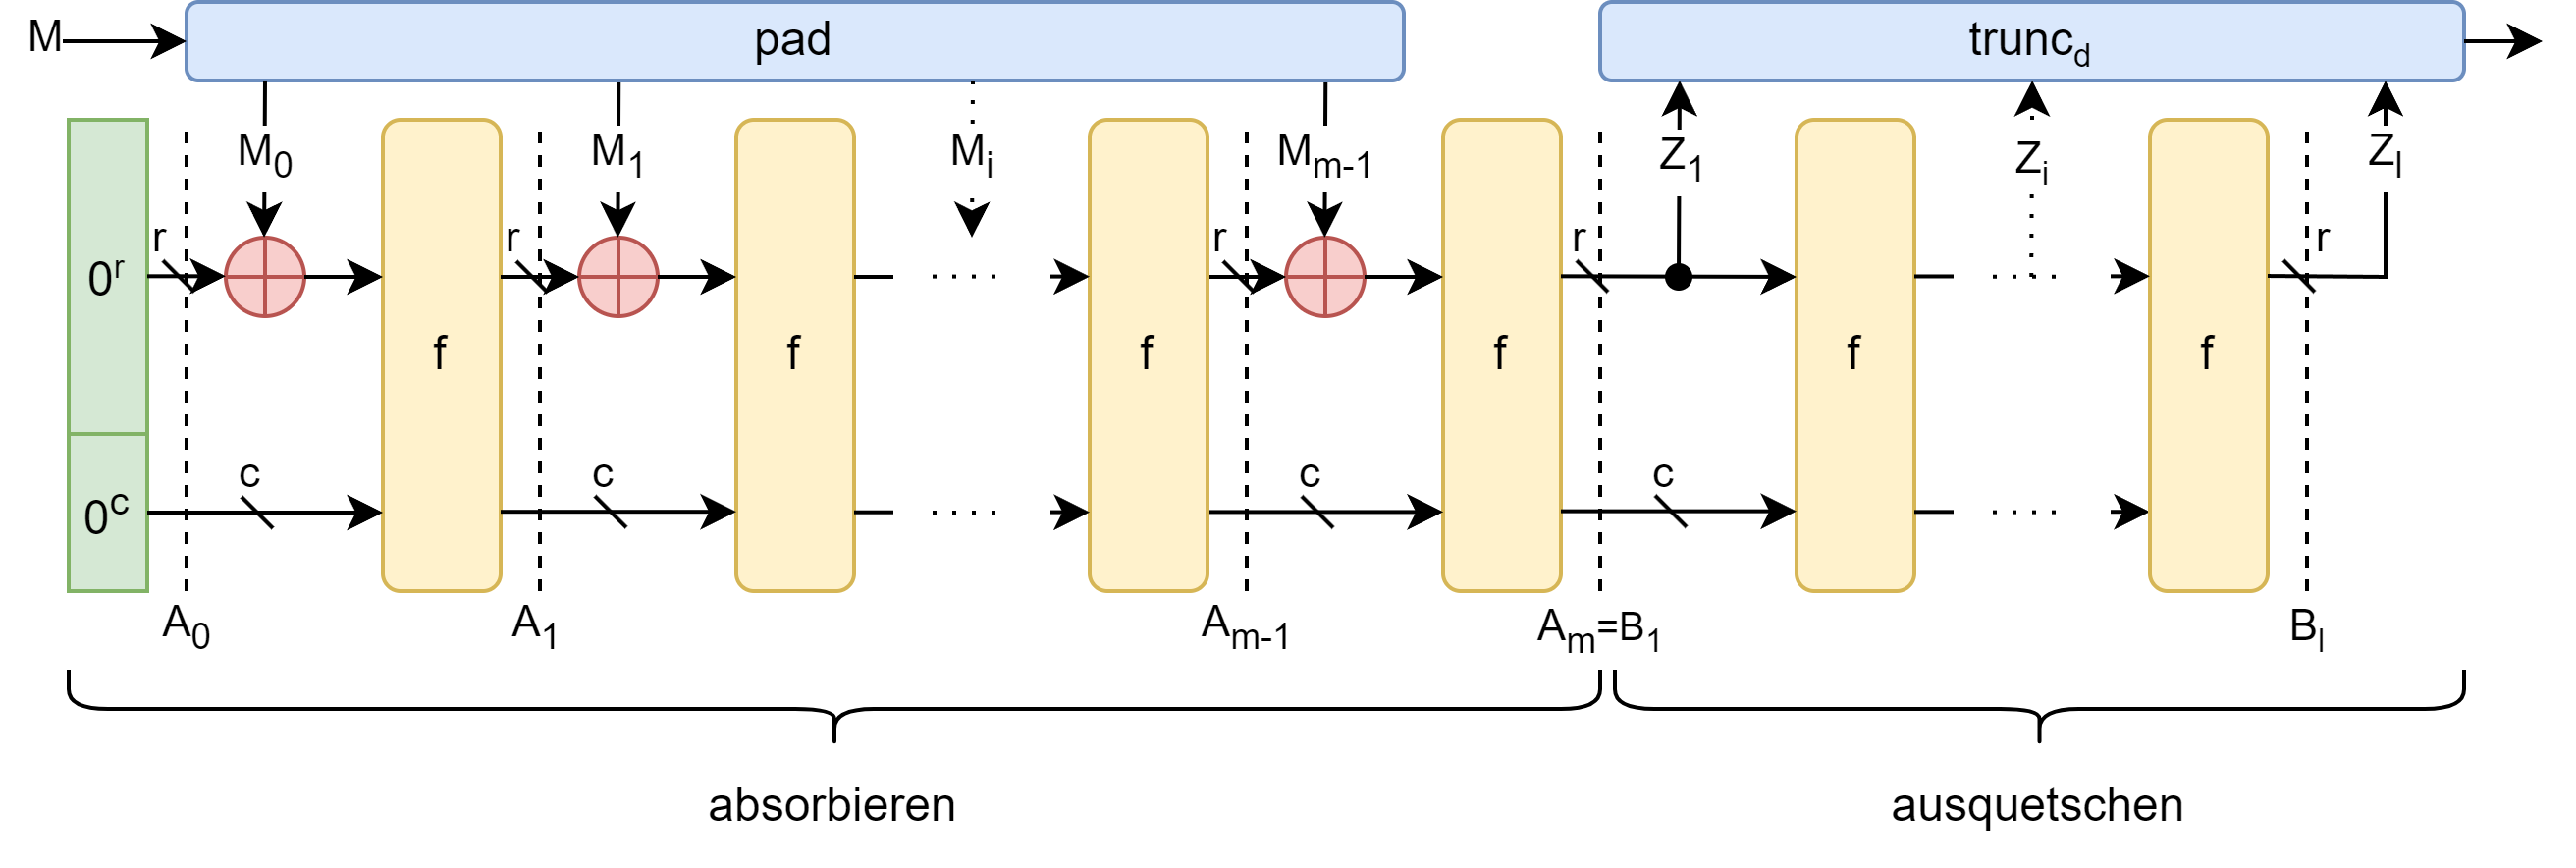
\includegraphics[scale=0.175]{images/Schwammkonstruktion.png}
    \caption{Aufbau der Schwammkonstruktion}
	(Nachbildung aus \cite{sha3-standard})
    \label{fig:schwammkonstruktion}
\end{figure}
Zur Komprimierung der Eingabe verwendet SHA-3 die sogenannte Schwammkonstruktion.
Sie erlaubt es eine Eingabe beliebiger Länge auf eine Ausgabe einer beliebigen anderen Länge d abzubilden.
Dazu wird die Eingabe, wie in Abbildung \ref{fig:schwammkonstruktion} veranschaulicht, erst mit Hilfe einer
Padding-Funktion in mehrere gleich große Blöcke einer festgelegten Länge aufgeteilt. Die Eingabeblöcke werden
dann der Reihe nach vom Schwamm "absorbiert". Danach werden auf ähnliche Weise die Ausgabeblöcke aus dem Schwamm "ausgequetscht".
Diese Ausgabeblöcke werden dann zur finalen Ausgabe zusammengesetzt. Wenn die Ausgabelänge kein Vielfaches der Blocklänge sein sollte, wird der Rest einfach abgeschnitten.
Die genaue Definition der Schwammkonstruktion über einer Transformation $f$ mit einer Padding-Funktion $pad$ sieht folgendermaßen aus:

\begin{align*}
    &\begin{alignedat}[t]{2}
        Seien\ & n \in \mathbb{N} && \text{ die Transformationsbreite}, \\
        & c \in \{1,...,n\} && \text{ die Kapazität (Anzahl "versteckter" Bits)}, \\
        & r \in \{1,...,n\} && \text{ die Blocklänge}, \\
        & M \in \{0,1\}^* && \text{ die zu verarbeitende Nachricht}, \\
        & m \in \mathbb{N} && \text{ die Anzahl an Blöcken, in die M eingeteilt wird}, \\
        & d \in \mathbb{N} && \text{ die gewünschte Ausgabe}, \\
        & l \coloneq \lceil \frac{d}{r} \rceil && \text{ die benötigte Blockanzahl an Ausgabe}, \\
        & pad: \mathbb{N}x\{0,1\}^* \to (\{0,1\}^r)^+ && \text{ eine Padding-Funktion}, \\
        & f: \{0,1\}^n \to \{0,1\}^n && \text{ eine Transformation}.
    \end{alignedat} \\
    \\
    &\text{Dann ist die Schwammkonstruktion } SPONGE[f,pad,c](M,d) \text{ definiert als:} \\
    &\begin{alignedat}[t]{3}
        SPONGE[f,pad,c](M, d) & \coloneq \mathbf{Z}[0] \mathbin\Vert ... \mathbin\Vert \mathbf{Z}[d-1]\ mit \\
        r & \coloneq 1600 - c \\
        M_1...M_{m} & \coloneq M \mathbin\Vert pad(r, M) \text{ wobei } |M_i| = r\ \forall i = 1,...,m\\
        \mathbf{A}_0 & \coloneq 0^n \\
        \mathbf{A}_i & \coloneq f(\mathbf{A}_{i-1} \oplus (M_{i-1} \mathbin\Vert 0^c))\ & \forall i = 1,...,m \\
        \mathbf{B}_1 & \coloneq \mathbf{A}_{m} \\
        \mathbf{B}_i & \coloneq f(\mathbf{B}_{i-1})\ & \forall i = 2,...,l \\
        \mathbf{Z}_i & \coloneq \mathbf{B}_i[0] \mathbin\Vert ... \mathbin\Vert \mathbf{B}_i[r-1] \\
        \mathbf{Z} & \coloneq \mathbf{Z}_1 \mathbin\Vert ... \mathbin\Vert \mathbf{Z}_l
    \end{alignedat}
\end{align*}
Die Kapazität $c$ bestimmt dabei wie viele Bits des internen Zustands $\mathbf{A}$ der Schwammkonstruktion von neuen Eingabeblöcken
nicht verändert werden dürfen. 
	
\subsection{SHA3-Hashfunktionen}
\label{cha:definition_sha3}
Die in Tabelle \ref{tab:uebersicht_sha3} aufgelisteten Hashfunktionen sind nun Instanzen dieser Schwammkonstruktion:
\begin{align*}
	\text{SHA3-224}(M) & \coloneq SPONGE[\text{KECCAK-p},pad10^*1, 448](M \mathbin\Vert 01, 224), \\
	\text{SHA3-256}(M) & \coloneq SPONGE[\text{KECCAK-p},pad10^*1, 512](M \mathbin\Vert 01, 256), \\
	\text{SHA3-384}(M) & \coloneq SPONGE[\text{KECCAK-p},pad10^*1, 768](M \mathbin\Vert 01, 256), \\
	\text{SHA3-512}(M) & \coloneq SPONGE[\text{KECCAK-p},pad10^*1,1024](M \mathbin\Vert 01, 512)
\end{align*}
Die zwei Extrabits "01", die an die Nachricht angefügt werden,
dienen nur dazu die erzeugten Hashes von den Ergebnissen anderer Betriebsmodi der KECCAK-p Permutation zu unterscheiden,
wie beispielsweise den beiden SHAKE-Funktionen.

\section{Sicherheitseigenschaften}
\label{cha:sha3_sicherheit}
Nun ist erstmal noch überhaupt nicht klar, wieso es sich bei den \ref{cha:definition_sha3} definierten Funktionen um eine Einwegfunktion handelt.
Schließlich verwendet sie eine sehr leicht invertierbare Permutation. Dazu wollen wir uns die Schwammkonstruktion noch einmal etwas genauer anschauen,
in diesem Fall am Beispiel von SHA3-256, wobei wir nur einen Block hashen. Um die Permutation invertieren zu können,
muss allerdings die gesamte Eingabe vorliegen. Da über den Hash $h$ einer Nachricht $M$ allerdings nur 256-Bit der Ausgabe der Permutation bekannt sind,
kann die Funktion nicht direkt invertiert werden. Auch kann nicht einfach eine beliebige Belegung für den restlichen Teil gewählt werden,
da am Ende nur ein Teil der Eingabe durch den Nachrichtenblock festgelegt werden kann. 
Die Schwierigkeit bei der Invertierung der Schwammfunktion entsteht also durch die Kombination aus Kapazität und dem Verwerfen eines Teils des Ergebnisses.
Diese Überlegung reicht natürlich noch nicht als Beweis, aber sie gibt einen intuitiven Einblick das zugrunde liegende Problem.
Bertoni et al. \cite{indifferentiability} bewiesen bereits, dass die Schwammkonstruktion selbst, wenn sie mit einer zufälligen Permutation initialisiert wird,
für einen klassischen Algorithmus von einem Zufallsorakel undifferenzierbar ist, eine Eigenschaft, die von Maurer et al. \cite{MaReHo04} eingeführt wurde als Generalisierung
der Ununterscheidbarkeit. Czajkowski \cite{quantum_indifferentiability} Zeigte außerdem, dass diese Eigenschaft auch für Quantenalgorithmen gilt. Undifferenzierbarkeit von einem Zufallsorakel
ist eine sehr starke Eigenschaft für kryptographische Systeme, da aus ihr direkt viele Sicherheitseigenschaften folgen \cite{indifferentiability}.
Damit diese Eigenschaft für SHA-3 gilt, muss allerdings die zugrundeliegende Permutation KECCAK-p ebenfalls undifferenzierbar von einer zufälligen Permutation sein.
Einen solchen Beweis gibt es bisher nicht. Allerdings ist beweisbar, dass KECCAK-p gegen alle bekannten Angriffe besteht, die zum Beispiel Techniken
wie die lineare oder differenzielle Kryptoanalyse verwenden \cite{Keccak11}.